% ============================================================
%  CHAPITRE 3 — RELEASE 1 : SOCLE FONCTIONNEL DE SMARTPM
% ============================================================
\chapter{Release 1 : Mise en place du socle fonctionnel de SmartPM}

\vspace{-0.3cm}
\begin{tcolorbox}[colback=lightgray, colframe=primaryblue,
  title=\textbf{Plan}, fonttitle=\bfseries]
  \begin{enumerate}[leftmargin=*, label=\arabic*.]
    \item Sprint 1 --- Authentification \& Gestion des utilisateurs
    \item Sprint 2 --- Gestion des projets \& Hi\'erarchie des t\^aches
    \item Sprint 3 --- Revues, Commentaires \& Notifications
  \end{enumerate}
\end{tcolorbox}

% ─────────────────────────────────────────────────────────
\section*{Introduction}
% ─────────────────────────────────────────────────────────

La premi\`ere release de SmartPM constitue le fondement sur lequel repose
l'ensemble de la plateforme. Elle a pour objectif d'\'etablir un socle
fonctionnel solide, s\'ecuris\'e et conforme aux exigences du d\'eveloppement
logiciel critique. Cette release couvre trois sprints d'une dur\'ee totale de
six semaines.

\vspace{0.3cm}

Pour chaque sprint, nous pr\'esenterons les objectifs, le backlog, la
sp\'ecification des besoins via un diagramme de cas d'utilisation, le
diagramme de classes, les diagrammes dynamiques (s\'equence, activit\'e,
\'etat), puis les interfaces r\'ealis\'ees.

% ═══════════════════════════════════════════════════════════
\newpage
\section{Sprint 1 : Authentification \& Gestion des utilisateurs}
\label{sec:s1}
% ═══════════════════════════════════════════════════════════

Ce premier sprint est consacr\'e \`a la mise en place de l'infrastructure
de s\'ecurit\'e et de gestion des identit\'es de SmartPM. Il constitue le
pr\'erequis indispensable de toutes les fonctionnalit\'es ult\'erieures.

\subsection{Objectifs du sprint 1}

L'objectif principal de ce sprint est de d\'evelopper un syst\`eme
d'authentification robuste et multi-m\'ethodes. Plus pr\'ecis\'ement, il
s'agit de :

\begin{itemize}
  \item Int\'egrer un syst\`eme d'authentification par tokens JWT
        (\textit{JSON Web Token}) avec gestion du refresh token (validit\'e
        15 minutes pour l'access token, 7 jours pour le refresh token).
  \item Impl\'ementer le protocole OAuth2 pour la connexion sociale
        via Google et GitHub.
  \item D\'efinir et appliquer une gestion fine des r\^oles utilisateurs :
        \textbf{ADMIN}, \textbf{MANAGER} et \textbf{MEMBER}.
  \item Mettre en place un seedage automatique du compte administrateur
        au premier d\'emarrage du backend (via \texttt{OnApplicationBootstrap}).
  \item D\'evelopper le module d'administration : CRUD complet sur les
        utilisateurs, consultation des journaux d'audit et r\'einitialisation
        des mots de passe.
\end{itemize}

\subsection{Backlog du sprint 1}

Le tableau~\ref{tab:backlog_s1} pr\'esente le backlog d\'etaill\'e du premier sprint.

\begin{table}[H]
\centering
\renewcommand{\arraystretch}{1.4}
\begin{tabularx}{\textwidth}{|c|X|c|c|}
\hline
\rowcolor{tablehead}
\textcolor{white}{\textbf{ID}} &
\textcolor{white}{\textbf{User Story}} &
\textcolor{white}{\textbf{Priorit\'e}} &
\textcolor{white}{\textbf{Charge (j)}} \\ \hline
US-1.1 & En tant qu'utilisateur, je peux m'inscrire avec email et mot de passe & Haute & 2 \\ \hline
US-1.2 & En tant qu'utilisateur, je peux me connecter via JWT (Login) & Haute & 2 \\ \hline
US-1.3 & En tant qu'utilisateur, je renouvelle mon token via le refresh token & Haute & 1 \\ \hline
US-1.4 & En tant qu'utilisateur, je me connecte via Google OAuth2 & Haute & 2 \\ \hline
US-1.5 & En tant qu'utilisateur, je me connecte via GitHub OAuth2 & Haute & 1 \\ \hline
US-1.6 & Le compte Admin est cr\'e\'e automatiquement au d\'emarrage & Haute & 1 \\ \hline
US-1.7 & En tant qu'Admin, je g\`ere les comptes utilisateurs (CRUD) & Moyenne & 3 \\ \hline
US-1.8 & En tant qu'Admin, je consulte les journaux d'audit & Moyenne & 2 \\ \hline
US-1.9 & En tant qu'Admin, je r\'einitialise le mot de passe d'un utilisateur & Faible & 1 \\ \hline
\end{tabularx}
\caption{Backlog du Sprint 1 --- Authentification \& Gestion des utilisateurs}
\label{tab:backlog_s1}
\end{table}

\subsection{Sp\'ecification des besoins fonctionnels}

\subsubsection{Identification des acteurs}

Trois acteurs interagissent avec le sous-syst\`eme d'authentification :
l'\textbf{Utilisateur non authentifi\'e} (peut s'inscrire et se connecter),
l'\textbf{Utilisateur authentifi\'e} (peut renouveler son token et se
d\'econnecter) et l'\textbf{Administrateur} (h\'erite des droits utilisateur
et dispose des fonctions d'administration).

\subsubsection{Diagramme de cas d'utilisation}

La figure~\ref{fig:uc_s1} repr\'esente les interactions entre les acteurs
et le sous-syst\`eme d'authentification de SmartPM.

\begin{figure}[H]
  \centering
  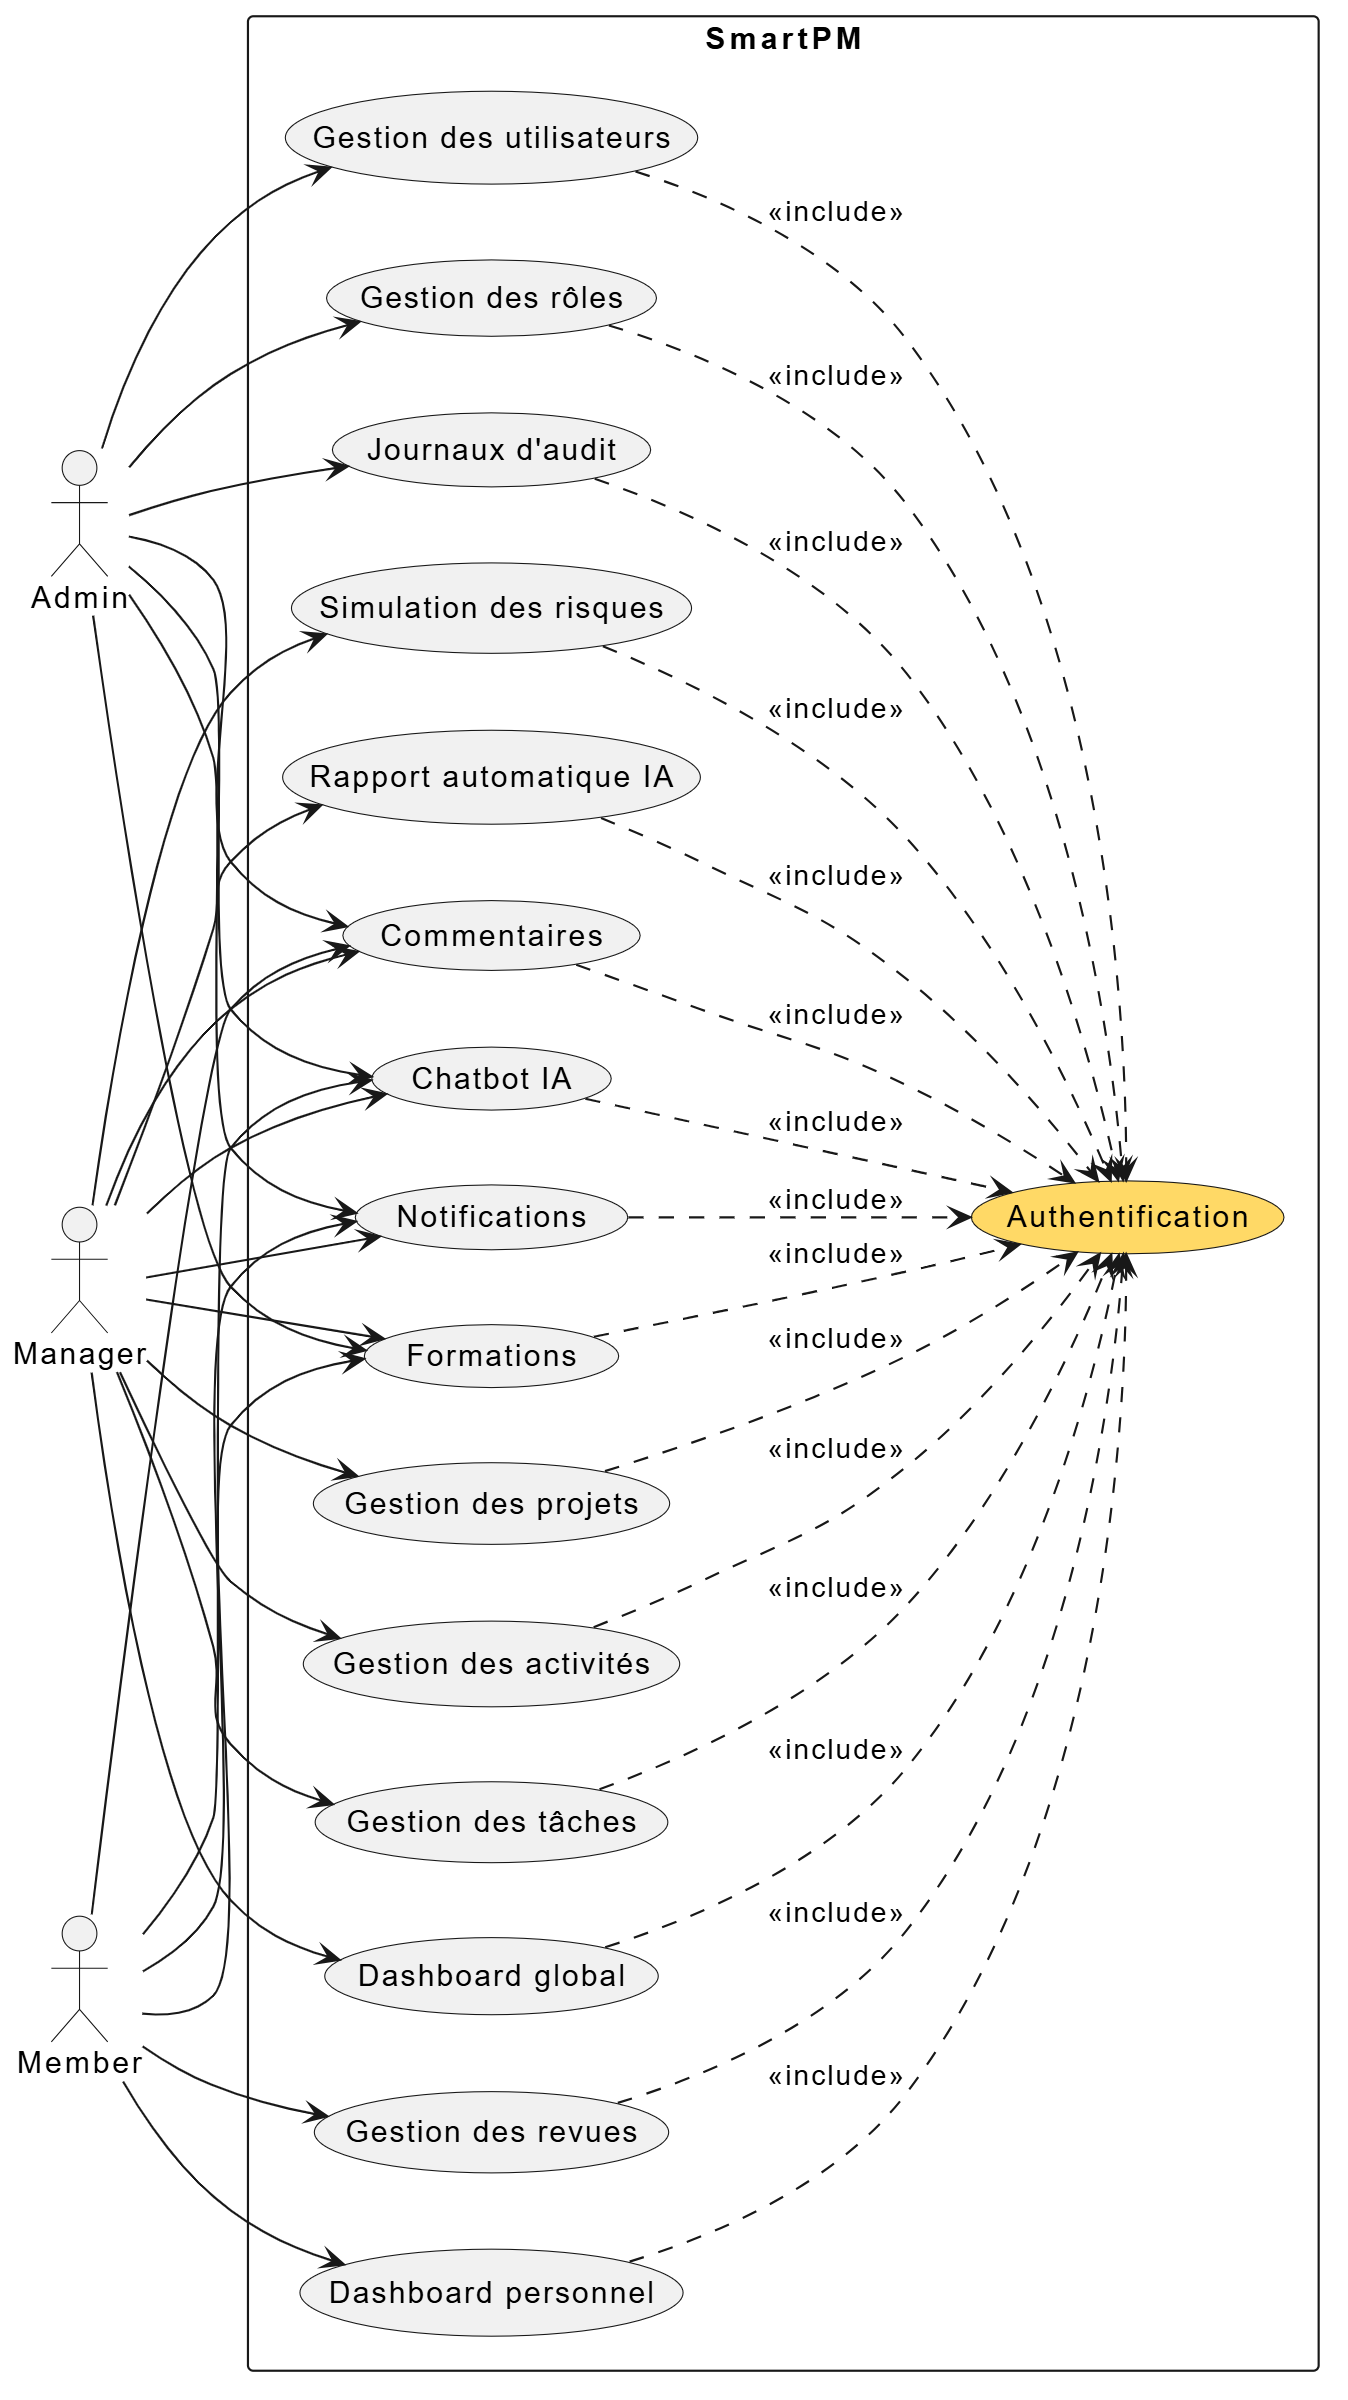
\includegraphics[width=\textwidth]{figures/chapter3/sprint1/uc_sprint1.png}
  \caption{Diagramme de cas d'utilisation --- Sprint 1}
  \label{fig:uc_s1}
\end{figure}

\subsection{Diagramme de classes du sprint 1}

La figure~\ref{fig:class_s1} pr\'esente le diagramme de classes du sprint 1.
Les entit\'es principales sont : \textbf{User} (email, passwordHash, role,
status, isOAuthUser), \textbf{RefreshToken} (token, userId, expiresAt,
isRevoked) et \textbf{AuditLog} (actorId, action, targetId, createdAt).

\begin{figure}[H]
  \centering
  \includegraphics[width=\textwidth]{figures/chapter3/sprint1/class_sprint1.png}
  \caption{Diagramme de classes --- Sprint 1}
  \label{fig:class_s1}
\end{figure}

\subsection{Diagrammes dynamiques du sprint 1}

\subsubsection{Diagramme de s\'equence --- Authentification JWT}

Le diagramme~\ref{fig:seq_jwt} illustre le flux complet d'authentification
par token JWT. L'utilisateur soumet son email et mot de passe depuis le
composant Angular \texttt{LoginComponent}. Le backend NestJS valide les
identifiants via la strat\'egie \texttt{LocalStrategy} de Passport.js,
compare le mot de passe avec le hash bcrypt stock\'e en base, puis g\'en\`ere
un access token (15 minutes) et un refresh token (7 jours). Le refresh token
est persist\'e dans MongoDB Atlas. Les requ\^etes ult\'erieures includent
l'access token dans l'en-t\^ete \texttt{Authorization: Bearer <token>}
inject\'e par un \texttt{HttpInterceptor} Angular.

\begin{figure}[H]
  \centering
  \includegraphics[width=\textwidth]{figures/chapter3/sprint1/seq_jwt.png}
  \caption{Diagramme de s\'equence --- Authentification JWT}
  \label{fig:seq_jwt}
\end{figure}

\subsubsection{Diagramme de s\'equence --- OAuth2 Social Login}

Le diagramme~\ref{fig:seq_oauth} illustre le flux d'autorisation OAuth2
(\textit{Authorization Code Flow}). Ce flux garantit que les identifiants
de l'utilisateur ne transitent jamais par le backend SmartPM. Apr\`es
redirection vers le fournisseur (Google ou GitHub), le profil r\'ecup\'er\'e
est upsert\'e dans MongoDB Atlas et un JWT SmartPM est g\'en\'er\'e.

\begin{figure}[H]
  \centering
  \includegraphics[width=\textwidth]{figures/chapter3/sprint1/seq_oauth2.png}
  \caption{Diagramme de s\'equence --- OAuth2 Social Login (Google / GitHub)}
  \label{fig:seq_oauth}
\end{figure}

\subsection{R\'ealisation du sprint 1}

\subsubsection{Architecture du module d'authentification}

Trois modules NestJS ont \'et\'e cr\'e\'es pour ce sprint :
\textbf{AuthModule} (orchestration JWT + OAuth2, endpoints
\texttt{/auth/login}, \texttt{/auth/register}, \texttt{/auth/refresh}),
\textbf{UserModule} (CRUD utilisateurs, sch\'ema Mongoose avec validation)
et \textbf{AdminModule} (prot\'eg\'e par \texttt{JwtAuthGuard} +
\texttt{RolesGuard(ADMIN)}, CRUD + audit logs).

\vspace{0.3cm}

Les mots de passe sont hash\'es avec \textbf{bcrypt} (facteur de co\^ut 12).
Trois strat\'egies Passport.js ont \'et\'e impl\'ement\'ees :
\texttt{LocalStrategy} (email/mot de passe), \texttt{JwtStrategy}
(v\'erification des tokens) et \texttt{GoogleStrategy}/\texttt{GitHubStrategy}
(OAuth2).

\subsubsection{Interfaces r\'ealis\'ees}

\begin{figure}[H]
  \centering
  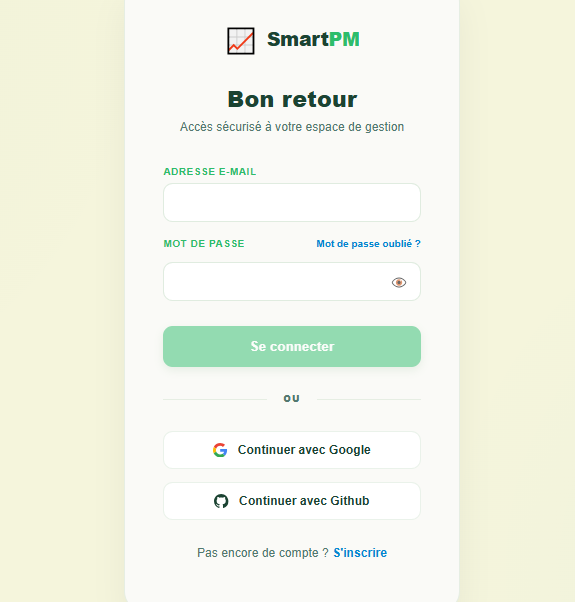
\includegraphics[width=0.8\textwidth]{images/screen_login.png}
  \caption{Interface de connexion de SmartPM}
  \label{fig:scr_login}
\end{figure}

\begin{figure}[H]
  \centering
  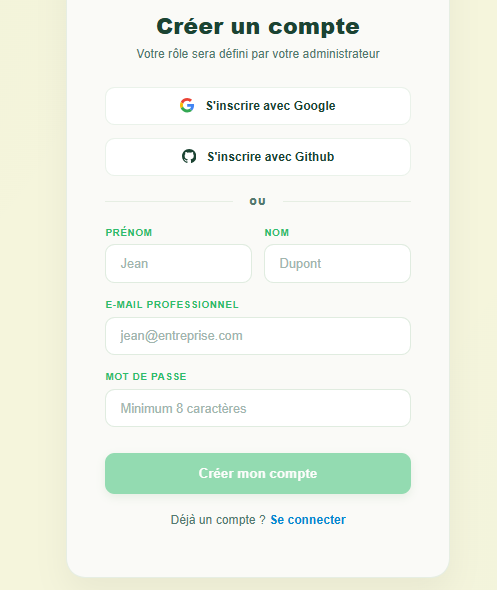
\includegraphics[width=0.8\textwidth]{images/screen_register.png}
  \caption{Interface d'inscription de SmartPM}
  \label{fig:scr_register}
\end{figure}

\begin{figure}[H]
  \centering
  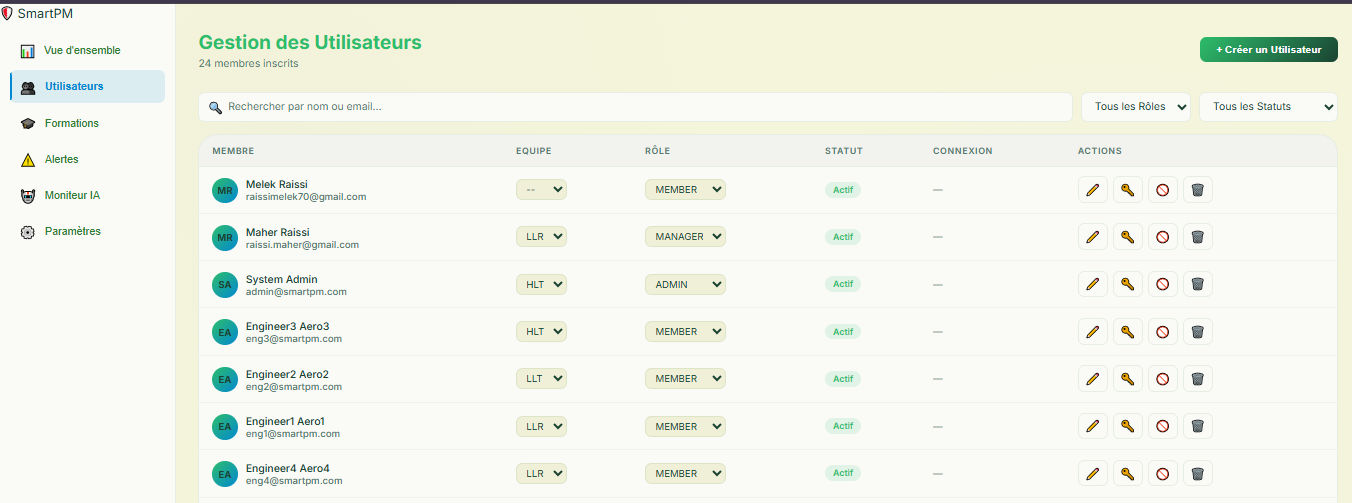
\includegraphics[width=\textwidth]{images/screen_admin_users.png}
  \caption{Module Admin --- Gestion des utilisateurs}
  \label{fig:scr_admin}
\end{figure}

\begin{figure}[H]
  \centering
  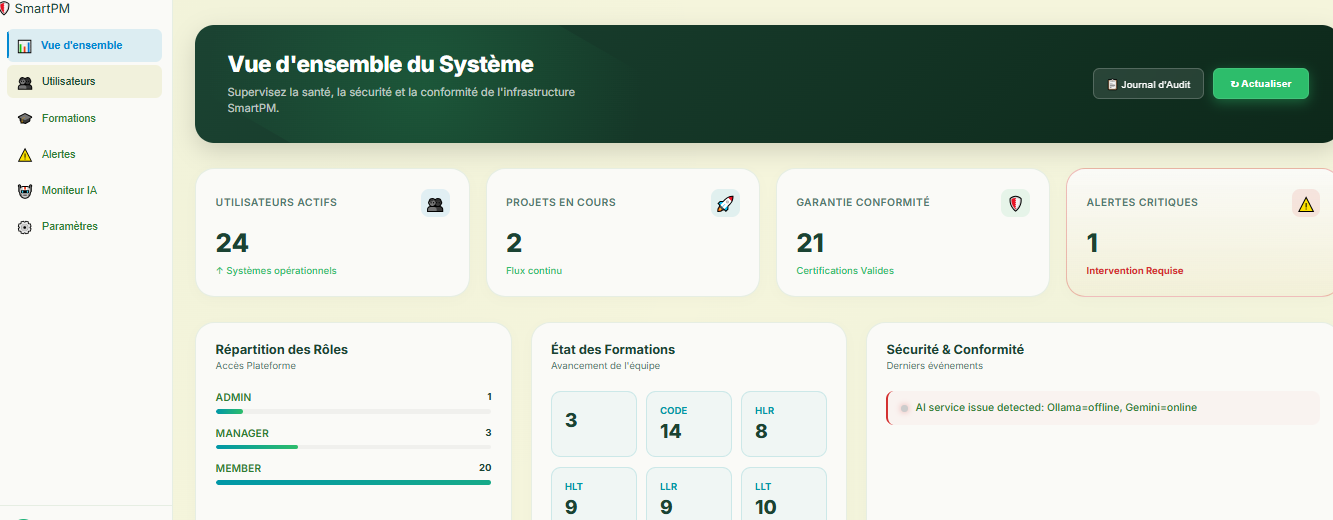
\includegraphics[width=\textwidth]{images/screen_audit_logs.png}
  \caption{Module Admin --- Journal d'audit des actions}
  \label{fig:scr_audit}
\end{figure}

% ═══════════════════════════════════════════════════════════
\newpage
\section{Sprint 2 : Gestion des projets \& Hi\'erarchie des t\^aches}
\label{sec:s2}
% ═══════════════════════════════════════════════════════════

Ce deuxi\`eme sprint constitue le c\oe ur m\'etier de SmartPM.
Il impl\'emente la structure de donn\'ees a\'eronautique conforme \`a
la norme DO-178C, qui impose une d\'ecomposition stricte du travail
en niveaux hi\'erarchiques.

\subsection{Objectifs du sprint 2}

\begin{itemize}
  \item Impl\'ementer le CRUD complet des projets avec un wizard
        multi-\'etapes (5 \'etapes).
  \item Mettre en place la hi\'erarchie \`a quatre niveaux :
        \textbf{Projet} $\rightarrow$ \textbf{Activit\'e} $\rightarrow$
        \textbf{Sous-Activit\'e} $\rightarrow$ \textbf{T\^ache}.
  \item G\'erer l'affectation des \'equipes et des membres aux projets.
  \item Impl\'ementer les \textit{Function Templates} (mod\`eles r\'eutilisables).
  \item D\'evelopper les tableaux de bord Manager et Member.
\end{itemize}

\subsection{Backlog du sprint 2}

\begin{table}[H]
\centering
\renewcommand{\arraystretch}{1.4}
\begin{tabularx}{\textwidth}{|c|X|c|c|}
\hline
\rowcolor{tablehead}
\textcolor{white}{\textbf{ID}} &
\textcolor{white}{\textbf{User Story}} &
\textcolor{white}{\textbf{Priorit\'e}} &
\textcolor{white}{\textbf{Charge (j)}} \\ \hline
US-2.1 & Manager : cr\'eer un projet (nom, description, dates, DAL) & Haute & 3 \\ \hline
US-2.2 & Manager : wizard multi-\'etapes de cr\'eation de projet & Haute & 4 \\ \hline
US-2.3 & Manager : CRUD des activit\'es d'un projet & Haute & 2 \\ \hline
US-2.4 & Manager : CRUD des sous-activit\'es & Haute & 2 \\ \hline
US-2.5 & Manager : CRUD des t\^aches avec affectation \`a un membre & Haute & 3 \\ \hline
US-2.6 & Manager : affecter une \'equipe \`a un projet & Haute & 2 \\ \hline
US-2.7 & Manager : cr\'eer et r\'eutiliser des Function Templates & Moyenne & 2 \\ \hline
US-2.8 & Manager : consulter le tableau de bord global & Haute & 3 \\ \hline
US-2.9 & Member : consulter son tableau de bord personnel & Haute & 2 \\ \hline
US-2.10 & Member : mettre \`a jour le statut d'une t\^ache & Haute & 1 \\ \hline
\end{tabularx}
\caption{Backlog du Sprint 2 --- Gestion des projets \& Hi\'erarchie des t\^aches}
\label{tab:backlog_s2}
\end{table}

\subsection{Sp\'ecification des besoins fonctionnels}

\subsubsection{Hi\'erarchie DO-178C dans SmartPM}

La norme DO-178C structure le d\'eveloppement logiciel en phases successives.
SmartPM traduit cette structure en quatre niveaux hi\'erarchiques :

\begin{itemize}
  \item \textbf{Projet} : Entit\'e racine repr\'esentant un programme
        logiciel a\'eronautique, associ\'e \`a une norme (DO-178C/DO-254)
        et un niveau de criticit\'e DAL (A \`a E).
  \item \textbf{Activit\'e} : Correspond \`a une phase majeure du cycle
        de vie (Requirements, Design, Coding, Testing).
  \item \textbf{Sous-Activit\'e} : D\'ecompose une activit\'e en travaux
        plus fins assignables \`a des individus sp\'ecifiques.
  \item \textbf{T\^ache} : Unit\'e atomique de travail, assign\'ee \`a un
        membre avec statut \texttt{TODO} $\rightarrow$ \texttt{IN\_PROGRESS}
        $\rightarrow$ \texttt{IN\_REVIEW} $\rightarrow$ \texttt{DONE}.
\end{itemize}

\subsubsection{Diagramme de cas d'utilisation}

\begin{figure}[H]
  \centering
  \includegraphics[width=\textwidth]{figures/chapter3/sprint2/uc_sprint2.png}
  \caption{Diagramme de cas d'utilisation --- Sprint 2}
  \label{fig:uc_s2}
\end{figure}

\subsection{Diagramme de classes du sprint 2}

La figure~\ref{fig:class_s2} pr\'esente le mod\`ele de donn\'ees du
sprint 2 : \textbf{Project} (m\'etadonn\'ees, DAL, norme),
\textbf{Team} (liste des membres), \textbf{Activity}, \textbf{SubActivity},
\textbf{Task} (assigneeId, status, priority, dueDate) et
\textbf{FunctionTemplate} (mod\`ele r\'eutilisable).

\begin{figure}[H]
  \centering
  \includegraphics[width=\textwidth]{figures/chapter3/sprint2/class_sprint2.png}
  \caption{Diagramme de classes --- Sprint 2}
  \label{fig:class_s2}
\end{figure}

\subsection{Diagrammes dynamiques du sprint 2}

\subsubsection{Diagramme de s\'equence --- Wizard de cr\'eation de projet}

Le \textit{Project Wizard} guide le Manager en 5 \'etapes :
(1)~Informations g\'en\'erales, (2)~Configuration normative (DAL, norme),
(3)~Structure des activit\'es, (4)~Constitution de l'\'equipe,
(5)~Confirmation. \`A l'\'etape finale, un \texttt{POST /projects} cr\'ee
le projet, ses activit\'es et affecte l'\'equipe en cascade.

\begin{figure}[H]
  \centering
  \includegraphics[width=\textwidth]{figures/chapter3/sprint2/seq_wizard.png}
  \caption{Diagramme de s\'equence --- Wizard de cr\'eation de projet}
  \label{fig:seq_wiz}
\end{figure}

\subsubsection{Diagramme d'activit\'e --- Cycle de vie d'une t\^ache}

\begin{figure}[H]
  \centering
  \includegraphics[width=\textwidth]{figures/chapter3/sprint2/activity_task.png}
  \caption{Diagramme d'activit\'e --- Cycle de vie d'une t\^ache}
  \label{fig:act_task}
\end{figure}

\subsection{R\'ealisation du sprint 2}

Cinq modules NestJS ont \'et\'e d\'evelopp\'es pour ce sprint :
\textbf{ProjectModule}, \textbf{ActivityModule}, \textbf{SubActivityModule},
\textbf{TaskModule} et \textbf{FunctionTemplateModule}. C\^ot\'e frontend,
quatre composants Angular ont \'et\'e cr\'e\'es :
\texttt{ProjectWizardComponent}, \texttt{ProjectDetailComponent},
\texttt{ManagerDashboardComponent} et \texttt{MemberDashboardComponent}.

\begin{figure}[H]
  \centering
  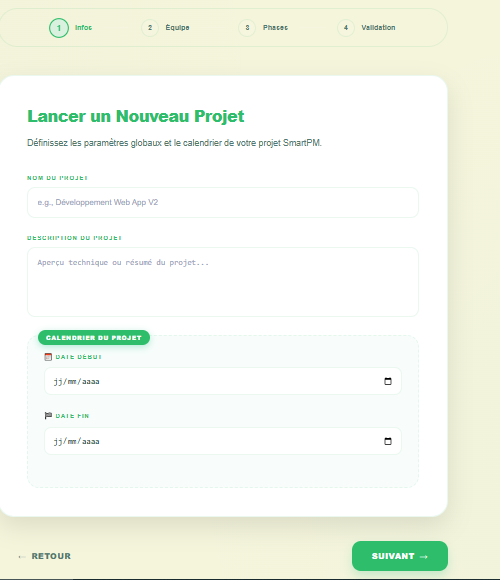
\includegraphics[width=0.85\textwidth]{images/screen_wizard_step1.png}
  \caption{Project Wizard --- \'Etape 1 : Informations g\'en\'erales}
  \label{fig:scr_wiz1}
\end{figure}

\begin{figure}[H]
  \centering
  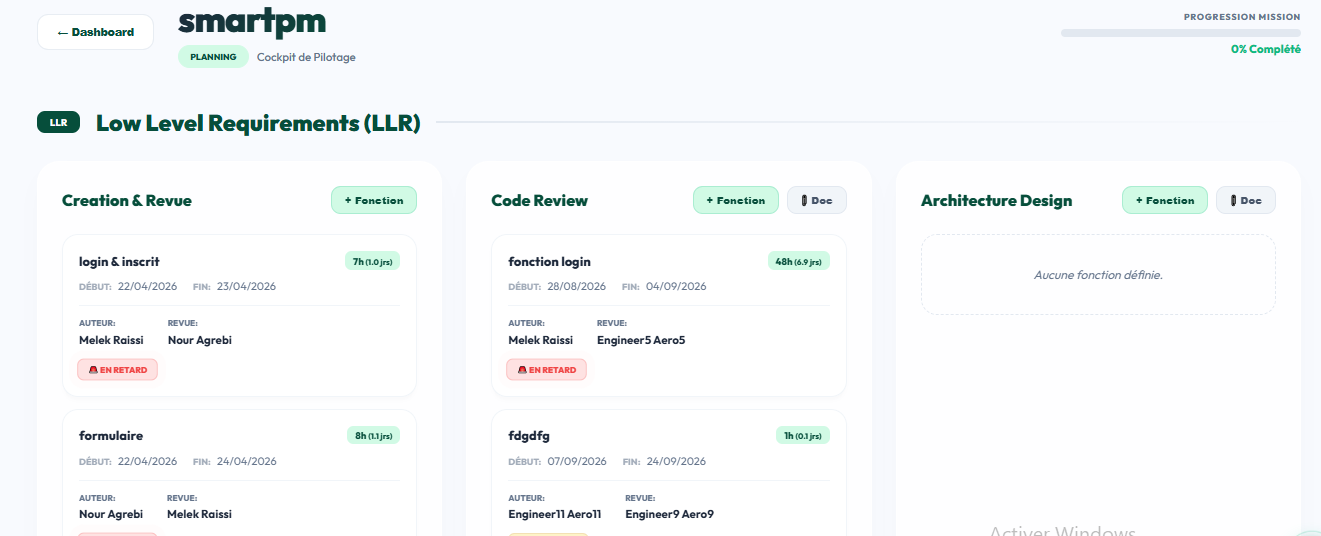
\includegraphics[width=\textwidth]{images/screen_project_detail.png}
  \caption{Vue d\'etaill\'ee d'un projet a\'eronautique SmartPM}
  \label{fig:scr_proj}
\end{figure}

\begin{figure}[H]
  \centering
  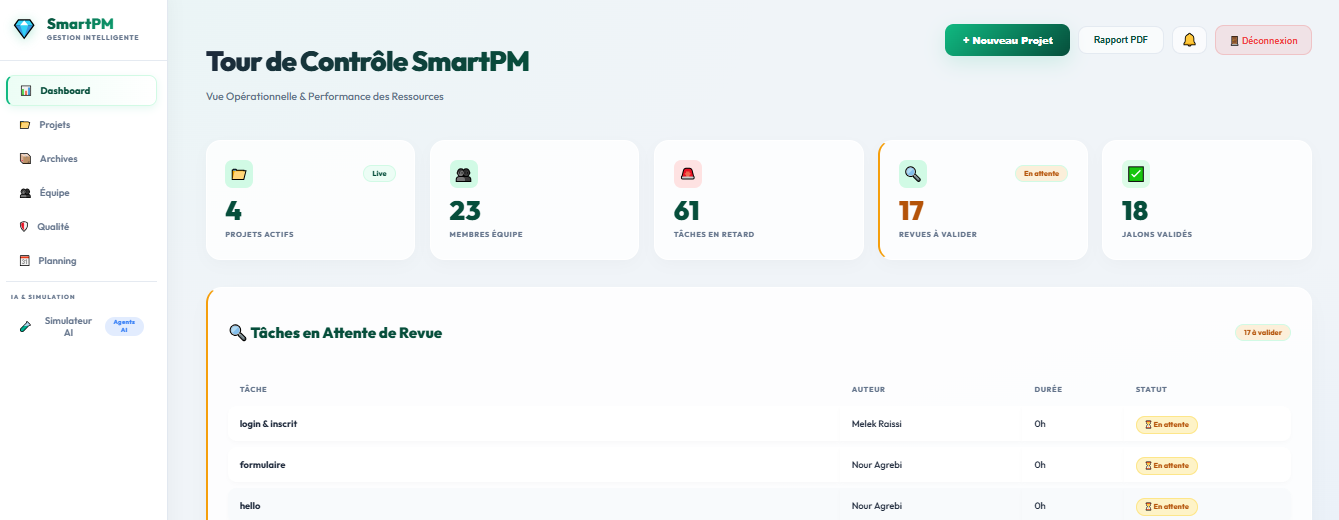
\includegraphics[width=\textwidth]{images/screen_manager_dashboard.png}
  \caption{Tableau de bord Manager --- Vue globale des projets}
  \label{fig:scr_mgr}
\end{figure}

\begin{figure}[H]
  \centering
  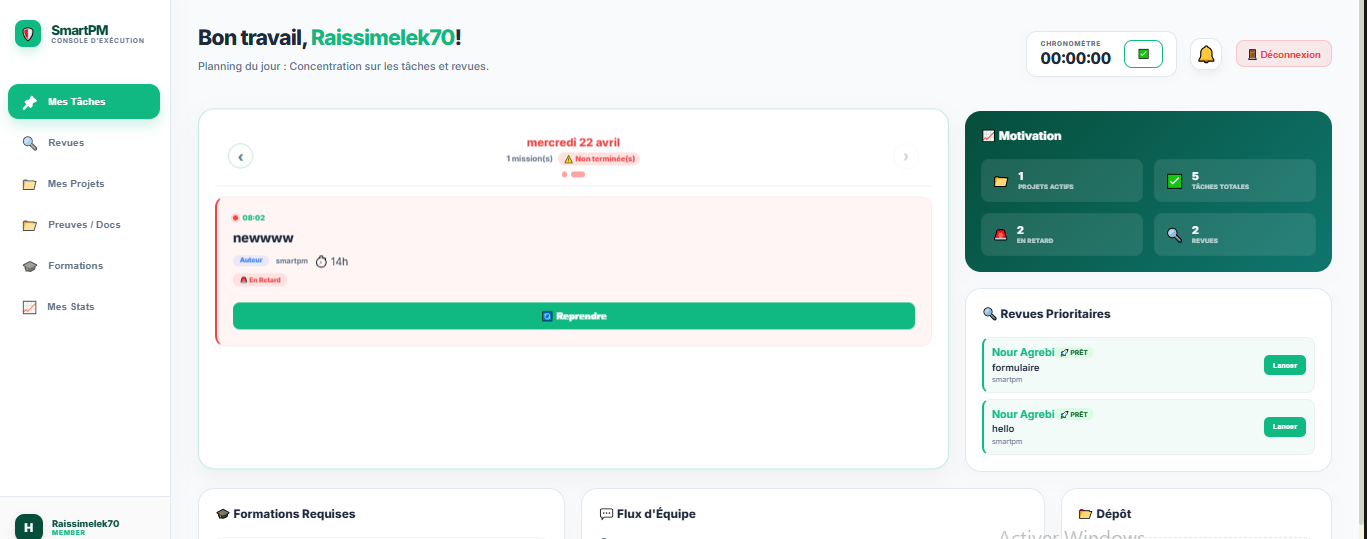
\includegraphics[width=\textwidth]{images/screen_member_dashboard.png}
  \caption{Tableau de bord Membre --- Vue personnelle des t\^aches}
  \label{fig:scr_mbr}
\end{figure}

% ═══════════════════════════════════════════════════════════
\newpage
\section{Sprint 3 : Revues, Commentaires \& Notifications}
\label{sec:s3}
% ═══════════════════════════════════════════════════════════

Ce troisi\`eme sprint enrichit SmartPM de m\'ecanismes de collaboration
et de contr\^ole qualit\'e conformes aux exigences DO-178C. La norme impose
que toute t\^ache soit r\'evis\'ee par une personne diff\'erente de son
auteur (\textbf{Author $\neq$ Reviewer}).

\subsection{Objectifs du sprint 3}

\begin{itemize}
  \item Impl\'ementer un syst\`eme de revues formelles avec la contrainte
        \textbf{Author $\neq$ Reviewer} (exigence DO-178C \S6.3).
  \item G\'erer le cycle de vie complet d'une revue :
        \texttt{PENDING} $\rightarrow$ \texttt{IN\_REVIEW} $\rightarrow$
        \texttt{APPROVED} ou \texttt{CHANGES\_REQUESTED}.
  \item Permettre aux membres de commenter les t\^aches (fil de discussion).
  \item Mettre en place des notifications en temps r\'eel via WebSockets.
  \item Impl\'ementer le suivi des certifications par phase DO-178C :
        HLR, LLR, CODE, LLT, HLT.
\end{itemize}

\subsection{Backlog du sprint 3}

\begin{table}[H]
\centering
\renewcommand{\arraystretch}{1.4}
\begin{tabularx}{\textwidth}{|c|X|c|c|}
\hline
\rowcolor{tablehead}
\textcolor{white}{\textbf{ID}} &
\textcolor{white}{\textbf{User Story}} &
\textcolor{white}{\textbf{Priorit\'e}} &
\textcolor{white}{\textbf{Charge (j)}} \\ \hline
US-3.1 & Member : soumettre une t\^ache \`a revue (Author $\neq$ Reviewer) & Haute & 3 \\ \hline
US-3.2 & Reviewer : approuver ou rejeter une revue avec commentaire & Haute & 2 \\ \hline
US-3.3 & Member : voir la liste des revues en attente & Haute & 1 \\ \hline
US-3.4 & Member : commenter une t\^ache (fil de discussion) & Moyenne & 2 \\ \hline
US-3.5 & Utilisateur : recevoir des notifications en temps r\'eel (WebSocket) & Haute & 3 \\ \hline
US-3.6 & Manager : valider une certification de phase (HLR/LLR/CODE/LLT/HLT) & Haute & 3 \\ \hline
US-3.7 & Member : voir son tableau de certifications par phase & Haute & 2 \\ \hline
\end{tabularx}
\caption{Backlog du Sprint 3 --- Revues, Commentaires \& Notifications}
\label{tab:backlog_s3}
\end{table}

\subsection{Sp\'ecification des besoins fonctionnels}

\subsubsection{La contrainte Author $\neq$ Reviewer dans DO-178C}

La norme DO-178C stipule dans sa section~6.3 que les activit\'es de
v\'erification doivent \^etre ind\'ependantes du processus de d\'eveloppement.
Dans SmartPM, cette contrainte est appliqu\'ee au niveau du service :
lors de l'assignation d'un reviewer, le \texttt{ReviewService} v\'erifie
que \texttt{authorId} $\neq$ \texttt{reviewerId}. Toute tentative
d'auto-assignation retourne une erreur HTTP~409 avec le message
\textit{<<~Un auteur ne peut pas r\'eviser sa propre t\^ache (DO-178C)~>>}.

\subsubsection{Diagramme de cas d'utilisation}

\begin{figure}[H]
  \centering
  \includegraphics[width=\textwidth]{figures/chapter3/sprint3/uc_sprint3.png}
  \caption{Diagramme de cas d'utilisation --- Sprint 3}
  \label{fig:uc_s3}
\end{figure}

\subsection{Diagramme de classes du sprint 3}

\begin{figure}[H]
  \centering
  \includegraphics[width=\textwidth]{figures/chapter3/sprint3/class_sprint3.png}
  \caption{Diagramme de classes --- Sprint 3}
  \label{fig:class_s3}
\end{figure}

\subsection{Diagrammes dynamiques du sprint 3}

\subsubsection{Diagramme d'\'etat --- Cycle de vie d'une revue}

Le diagramme~\ref{fig:state_rev} illustre les transitions d'\'etat d'une
revue de t\^ache. Une revue commence dans l'\'etat \texttt{PENDING} d\`es
la soumission. Le reviewer la passe \`a \texttt{IN\_REVIEW}, puis soit
\texttt{APPROVED} (t\^ache $\rightarrow$ DONE) soit
\texttt{CHANGES\_REQUESTED} (retour \`a l'auteur pour correction).

\begin{figure}[H]
  \centering
  \includegraphics[width=\textwidth]{figures/chapter3/sprint3/state_review.png}
  \caption{Diagramme d'\'etat --- Cycle de vie d'une revue DO-178C}
  \label{fig:state_rev}
\end{figure}

\subsubsection{Diagramme de s\'equence --- Soumission et traitement d'une revue}

\begin{figure}[H]
  \centering
  \includegraphics[width=\textwidth]{figures/chapter3/sprint3/seq_review.png}
  \caption{Diagramme de s\'equence --- Soumission et traitement d'une revue}
  \label{fig:seq_rev}
\end{figure}

\subsection{R\'ealisation du sprint 3}

Quatre modules NestJS ont \'et\'e d\'evelopp\'es :
\textbf{ReviewModule} (endpoints \texttt{/reviews}, v\'erification
Author~$\neq$~Reviewer, transitions d'\'etat),
\textbf{CommentModule} (fil de discussion par t\^ache),
\textbf{NotificationModule} (\texttt{@WebSocketGateway} avec
\texttt{socket.io}, \'ev\'enements \texttt{task.assigned},
\texttt{review.requested}, \texttt{review.approved}) et
\textbf{CertificationModule} (suivi des phases HLR/LLR/CODE/LLT/HLT,
validation par Manager ou Admin).

\begin{figure}[H]
  \centering
  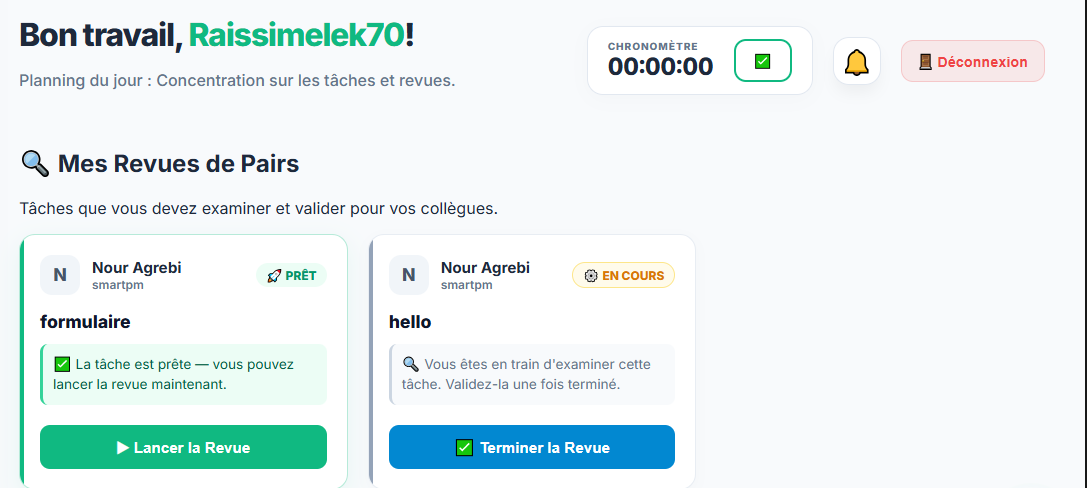
\includegraphics[width=0.85\textwidth]{images/screen_review_form.png}
  \caption{Interface --- Formulaire de revue (contrainte DO-178C)}
  \label{fig:scr_revform}
\end{figure}

\begin{figure}[H]
  \centering
  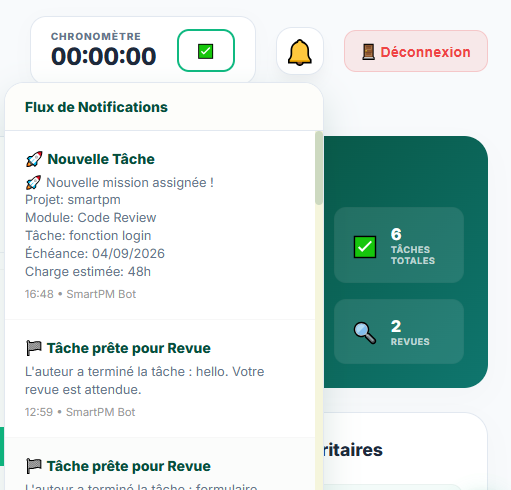
\includegraphics[width=0.8\textwidth]{images/screen_notifications.png}
  \caption{Panneau de notifications en temps r\'eel (WebSocket)}
  \label{fig:scr_notif}
\end{figure}

\begin{figure}[H]
  \centering
  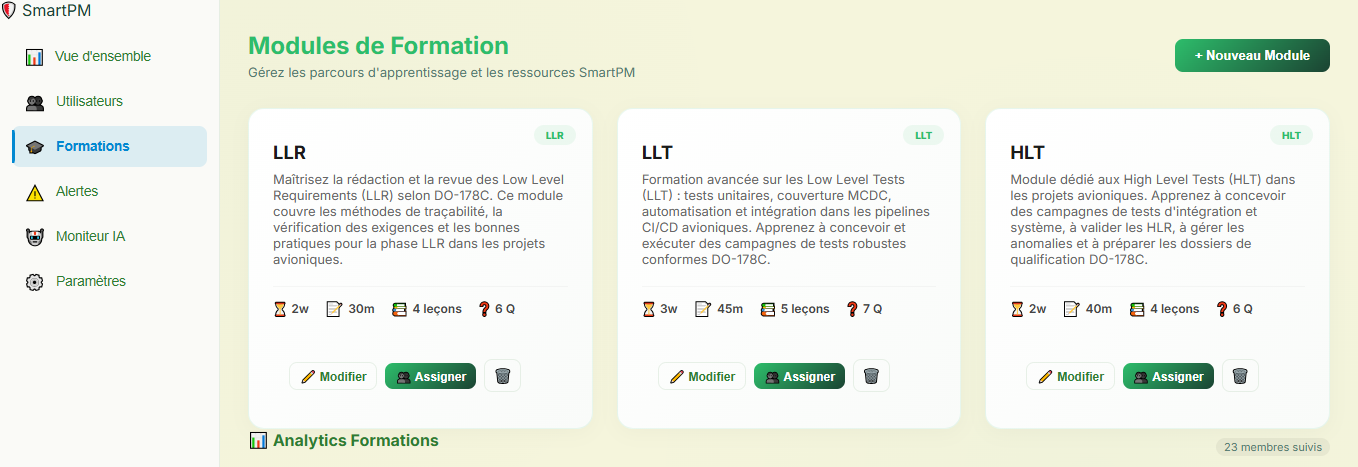
\includegraphics[width=\textwidth]{images/screen_certifications.png}
  \caption{Tableau de certifications par phase DO-178C}
  \label{fig:scr_certif}
\end{figure}

% ─────────────────────────────────────────────────────────
\section*{Conclusion}
% ─────────────────────────────────────────────────────────

Au terme de cette premi\`ere release, les fondations fonctionnelles de
SmartPM sont pleinement op\'erationnelles. Le syst\`eme d'authentification
multi-m\'ethodes garantit la s\'ecurit\'e des acc\`es, la hi\'erarchie de
gestion des projets refl\`ete fid\`element les exigences DO-178C, et les
m\'ecanismes de revues et de notifications assurent une collaboration
fluide et tra\c{c}able entre les membres de l'\'equipe.

\vspace{0.3cm}

Le chapitre suivant pr\'esentera la deuxi\`eme release, qui apporte
l'intelligence artificielle et l'infrastructure DevOps compl\`ete pour
garantir la haute disponibilit\'e de la plateforme.
